\chapter{One Dimensional Deterministic Case}\label{chap:oned-deterministic}

\todo[inline]{Change domain notation}

The simplest form of Laplace's Equation we can consider is the one dimensional
case where the coefficients are deterministic in which case the equation is
given by:

\begin{equation}\label{eq:oned-deterministic}
\begin{aligned}
    -au''(x) + bu'(x) + cu(x) &= f(x) &\text{ in } \Omega = [0, 1] \\
                         u(x) &= 0 &\text{ on } \delta\Omega = \{0, 1\}
\end{aligned}
\end{equation}

We consider the equation in the interval $[0,1]$ and prescribe a zero Dirichlet
condition at the endpoints $x = 0$ and $x = 1$.

\todo[inline]{In the deterministic case, we should be able to solve various
versions of this analytically. Include a few such cases and their solutions
they will provide us with a few good examples to compare our numerical
solutions with}

\section{Weak Formulation}

\todo[inline]{Give proper definitions of $V$ and $W$}
\todo[inline]{Justify the necessity of the weak formulation}

The first step in implementing the finite element method is to obtain the weak
formulation of this problem. To get the continuous weak form of the equation,
we multiply through by $v \in W$ and integrate over the domain:

\begin{equation}
    -a\int_0^1{u''(x)v(x)\ dx} + b\int_0^1{u'(x)v(x)\ dx}
    + c\int_0^1{u(x)v(x)\ dx} = \int_0^1{f(x)v(x)\ dx}
\end{equation}

Integrating the first term by parts gives us:

\begin{equation}
    -a\int_0^1{u''(x)v(x)\ dx} = -a\underbrace{[ u'(x)v(x) ]_0^1}_{ = 0}
    + a\int_0^1{u'(x)v'(x)\ dx}
\end{equation}

Where the underbraced term is zero as $v$ is zero at the endpoints of the
domain. Hence the continuous weak form of \myref{eq:oned-deterministic} is given
by:

\begin{equation}\label{eq:wk-oned-deterministic}
    a\int_0^1{u'(x)v'(x)\ dx} + b\int_0^1{u'(x)v(x)\ dx}
    + c\int_0^1{u(x)v(x)\ dx} = \int_0^1{f(x)v(x)\ dx}
\end{equation}

And a weak solution would be to find $u \in V$ such that, the above equation is
satisfied $\forall v \in W$

\section{Discrete Formulation}

\begin{figure}
\centering
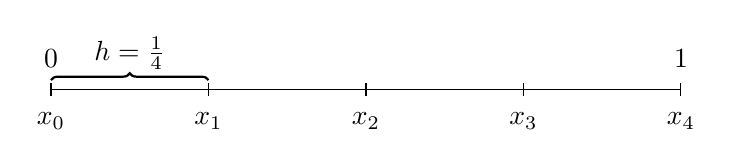
\begin{tikzpicture}[scale=8]
    % Draw the 0-1 interval
    \draw (0,0) -- (1, 0);

    % Draw the 'ticks' along the axis as well as the labels
    \foreach \x in {0,...,4}
    {
        \draw (0.25*\x, 0.01) -- (0.25*\x, -0.01);
        \node (\x) at (0.25*\x, -0.05) {$x_\x$};
    }

    % Draw the 0, 1 labels
    \node () at (0, 0.05) {0};
    \node () at (1, 0.05) {1};

    % Finally demonstrate the length of the interval
    \draw[thick, decoration={brace}, decorate] (0, 0.015) -- (0.25, 0.015)
        node[pos=0.5, anchor=south] {$h = \frac{1}{4}$};
\end{tikzpicture}


\caption{Example discretisation with N = 4}
\label{fig:one-d-discretisation}
\end{figure}

For a given parameter $N \in \mathbb{N}$ we define $N+1$ equally spaced nodes
$x_i$ $i \in \{0, \ldots, N\}$ in the interval $[0,1]$ where
$x_0 = 0, x_N = 1$. Then we can divide the domain into $N$ subintervals
$ I_i = [x_i, x_{i+1}]$, $i \in \{0,\ldots,N - 1\}$ of length $h = \frac{1}{N}$.
We can then define our discretisation to be:

\[
    D^h = \bigcup_{i=0}^{N - 1} I_i
\]

See Figure \ref{fig:one-d-discretisation} for an example discretisation
when $N=4$.  Upon such a discretisation we can define suitable finite
dimensional subspaces of our trial and test spaces $V^h \subset V$, $W^h
\subset W$.

\begin{align*}
    V^h &= \{v \in V: v \text{ is linear on } I_i,
          \ i \in \{0, \ldots, N - 1\},
          v \text{ is continuous on } [0, 1]\} \\
    W^h &= \{w \in W: w \text{ is linear on } I_i,
          \ i \in \{0, \ldots, N - 1\},
          w \text{ is continuous on } [0, 1]\}
\end{align*}

By choosing appropriate basis functions $\phi_i$ that span the space, we will
be able to approximate the solution as such:

\begin{equation}\label{eq:one-d-approx-soln}
    u^h(x) = \sum_{j = 0}^N{u_j\phi_j(x)}
\end{equation}

where $u_i$ will be the approximate value of the solution at the node $x_i$. In
a similar manner we will also be able to approximate $f(x)$:

\begin{equation}
    f(x) \approx \sum_{j = 0}^N f_j\phi_j(x)
\end{equation}

where $f_i = f(x_i)$. By writing the functions $u$ and $f$ in terms of their
values at the nodes $x_i$ then by taking a sufficiently large number of nodes
we can approximate them to within an acceptable margin of error.

\todo[inline]{Give an estimate for the error of the FEM for this problem -
Use the book!!}
\todo[inline]{Possibly include mention of existence and uniqueness of the
solution - Use the book !!}

An appropriate basis would be the so called `hat functions' which we can define
for each interior node as follows:

\begin{equation}\label{eq:one-d-hat-basis}
    \phi_i(x) = \left\{\begin{array}{c c}
                    \frac{x - x_{i-1}}{x_i - x_{i - 1}}, & x \in [x_{i-1}, x_i] \\
                    \frac{x_{i+1} - x}{x_{i + 1} - x_i}, & x \in [x_i, x_{i + 1}] \\
                    0, & \text{otherwise}
                \end{array}\right.
\end{equation}

And in the special case of the boundary nodes $x_0$ and $x_N$ we only consider
the intervals which lie in our domain:

\begin{align}
    \phi_0(x) &= \left\{\begin{array}{c c}
                    \frac{x_1 - x}{x_1 - x_0}, & x \in [x_0, x_1] \\
                    0, & \text{otherwise}
    \end{array}\right.
    \\
    \phi_N(x) &= \left\{\begin{array}{c c}
                    \frac{x - x_{N - 1}}{x_N - x_{N-1}}, & x \in [x_{N-1}, x_N] \\
                    0, & \text{otherwise}
    \end{array}\right.
\end{align}

As the weak formulation \myref{eq:wk-oned-deterministic} must be satisfied for
all $v \in W$ then in particular it must be satisfied for the basis functions
$\phi_i(x)$. So by taking $v = \phi_i(x)$ for each $i \in \{1,\ldots,N\}$ and
substituting our approximations for $u$ and $f$ we obtain:

\begin{align*}
    a\int_0^1{\left(\sum_{j = 0}^N{u_j\phi_j(x)}\right)'\phi_i'(x)\, dx}
    &+b\int_0^1{\left(\sum_{j = 0}^N{u_j\phi_j(x)}\right)'\phi_i(x)\, dx} \\
    &+c\int_0^1{\left(\sum_{j = 0}^N{u_j\phi_j(x)}\right)\phi_i(x)\, dx} =
    \int_0^1{\left(\sum_{j = 0}^Nf_j\phi_j(x)\right)\phi_i(x)\, dx}
\end{align*}

By the linearity of the integrals and derivatives we can write this as:

\begin{align*}
    a\sum_{j = 0}^Nu_j\int_0^1\phi_i'(x)\phi_j'(x)\, dx
    &+b\sum_{j = 0}^Nu_j\int_0^1\phi_i(x)\phi_j'(x)\, dx \\
    &+c\sum_{j = 0}^Nu_j\int_0^1\phi_i(x)\phi_j(x)\, dx =
    \sum_{j = 0}^Nf_j\int_0^1\phi_i(x)\phi_j(x)\, dx
\end{align*}

for each $i \in \{1,\ldots,N\}$. Or equivalently:

\begin{align}\label{eq:oned-deterministic-discrete}
  \begin{split}
    \sum_{j = 0}^N\underbrace{\left(a\int_0^1\phi_i'(x)\phi_j'(x)\, dx
        + b\int_0^1\phi_i(x)\phi_j'(x)\, dx + c\int_0^1\phi_i(x)\phi_j(x)\, dx\right)}_{:= A_{i,j}}u_j  \\
    = \sum_{j = 0}^N\underbrace{\int_0^1{\phi_i(x)\phi_j(x)}\, dx}_{:= M_{i,j}}f_j
  \end{split}
\end{align}

This effectively reduces the weak formulation \myref{eq:wk-oned-deterministic}
to a linear system $Au^h = Mf$ where $A$ is known as the stiffness matrix and
$M$ is known as the mass matrix. Being a linear system it is relatively
straightforward to solve solve computationally for the unknown vector $u^h$ and
by taking a sufficiently fine discretisation we can achieve a good
approximation to the actual solution $u$.

\begin{equation}
    \sum_{j=0}^NA_{i,j}u_i = \sum_{j=0}^NM_{i,j}f_i,\ i \in \{0,\ldots,N\}
\end{equation}

However due to the Dirichlet condition we have in \myref{eq:oned-deterministic}
we already know the value of $u$ at the nodes $x_0$ and $x_N$ so in the cases
where $j = 0$ and $j = N$ the associated terms on the left hand side can be
removed from the system of equations. Furthermore as we knows the value of our
solution $u$ at these nodes, we can move the associated terms over to the right
hand side:

\begin{equation}
    \sum_{j=1}^{N-1}A_{i,j}u_i =
        \sum_{j=1}^{N}M_{i,j}f_j - A_{i,0}u(0) - A_{i,N}u(1)
\end{equation}

In our particular problem we have a zero Dirichlet condition so the linear
system reduces quite nicely to:

\begin{equation}\label{eq:oned-deterministic-fem}
    \sum_{i=1}^{N-1}\sum_{j=1}^{N-1}A_{i,j}u_j
        = \sum_{i=1}^{N-1}\sum_{j=0}^NM_{i,j}f_j,\ i \in \{1,\dots,N-1\}
\end{equation}

Solving this system for the vector $\v{u}$ will give us the approximate
solution to the equation \myref{eq:oned-deterministic}

\section{Constructing the Global Linear System}\label{sec:oned-deterministic-global-construct}

The final step in implementing the finite element method is to assemble the
global system of equations i.e.  determining the entries of $A_{i,j}$ and
$M_{i,j}$ which we currently have written in terms of a number of integrals
\myref{eq:oned-deterministic-discrete}. Due to the fact that our domain has
been subdivided into many subintervals we can consider the contribution from
each and combine them later into the global system.

\begin{figure}
\centering
\begin{tikzpicture}[scale=6]

    % Draw the axis
    \draw[thin] (-1.25, 0) -- (1.25, 0);

    % Draw the endpoints
    \draw (-1.25, 0.02) -- (-1.25, -0.02);
    \draw (1.25, 0.02) -- (1.25, -0.02);
    \node (0) at (-1.25, -0.07) {$x_0$};
    \node (N) at (1.25, -0.07) {$x_N$};

    % Draw the dot dot dots
    \node (1) at (-1, -0.07) {$\cdots$};
    \node (2) at (1, -0.07) {$\cdots$};

    % Draw the supporting nodes
    \draw (-0.75, 0.02) -- (-0.75, -0.02);
    \draw (0.75, 0.02) -- (0.75, -0.02);
    \node (k0) at (-0.75, -0.07) {$x_{k-1}$};
    \node (k3) at (0.75, -0.07) {$x_{k+2}$};

    % Draw the intervals we are interested in
    \draw (-0.25, 0.02) -- (-0.25, -0.02);
    \draw (0.25, 0.02) -- (0.25, -0.02);
    \draw[dotted] (-0.25, 0) -- (-0.25, 0.5);
    \draw[dotted] (0.25, 0) -- (0.25, 0.5);
    \node (k1) at (-0.25, -0.07) {$x_k$};
    \node (k2) at (0.25, -0.07) {$x_{k + 1}$};

    % Finally draw the two basis functions of interest
    \draw[dashed] (-0.75, 0) -- (-0.25, 0.5);
    \draw (-0.25, 0.5) -- (0.25, 0);
    \draw[red] (-0.25, 0) -- (0.25, 0.5);
    \draw[red,dashed] (0.25, 0.5) -- (0.75, 0);
    \node[anchor=east] (p1) at (-0.25, 0.51) {$\phi_k$};
    \node[anchor=west] (p2) at (0.25, 0.51) {\color{red}$\phi_{k+1}$};
    \node[anchor=north] (ps1) at (-0.1, 0.5) {$\psi_{k,1}$};
    \node[anchor=north] (ps2) at (0.1, 0.5) {\color{red}$\psi_{k,2}$};

\end{tikzpicture}


\caption{Example of the local basis functions $\psi_{k,1}$ and $\psi_{k,2}$
         in the interval $[x_k, x_{k + 1}]$}
\label{fig:oned-local-basis}
\end{figure}

Consider a subinterval $[x_k, x_{k+1}]$, as we can see in Figure
\ref{fig:oned-local-basis} due to the compact support of the global basis
functions $\phi_i$ each subinterval will have 2 local basis functions which we
will call $\psi_{k,1}$ and $\psi_{k,2}$ associated with it which we write as
follows:

\begin{equation}
    \psi_{k,1}(x) = \frac{x_{k+1} - x}{x_{k+1} - x_k}
\end{equation}

\begin{equation}
    \psi_{k,2}(x) = \frac{x - x_k}{x_{k+1} - x_k}
\end{equation}

where the index $k$ corresponds with the index of the starting node of the
interval $x_k$.  This means we can write any function $v \in V^h$ locally in
the subinterval $[x_k, x_{k+1}]$ as:

\begin{align*}
    v(x) = v(x_k)\psi_{k,1}(x) + v(x_{k+1})\psi_{k,2}(x)
\end{align*}

which means locally we can rewrite \myref{eq:oned-deterministic-discrete} as

\begin{equation}\label{eq:oned-deterministic-local-discrete}
  \begin{split}
    \sum_{r = 1}^2\sum_{s = 1}^2\underbrace{\left(
          a\int_{x_k}^{x_{k+1}}\psi_{k,r}'(x)\psi_{k,s}'(x)\, dx
        + b\int_{x_k}^{x_{k+1}}\psi_{k,r}'(x)\psi_{k,s}(x)\, dx
        + c\int_{x_k}^{x_{k+1}}\psi_{k,r}(x)\psi_{k,s}(x)\, dx
    \right)}_{A^{(k)}_{r,s}}u_r  \\
    = \sum_{r= 1}^2\sum_{s = 1}^2\underbrace{
            \int_{x_k}^{x_{k+1}}{\psi_{k,r}(x)\psi_{k,s}(x)}\, dx}_{M^{(k)}_{r,s}}f_r
  \end{split}
\end{equation}

where we now denote these $2 \times 2$ matrices by $A^{(k)}_{r,s}$ and
$M^{(k)}_{r,s}$ which are called the local stiffness and mass matrices
respectively. As we can see from the above, we will need the derivatives of
these local basis functions which are given by:

\begin{align}
  \begin{split}
    \psi_{k,1}'(x) &= \frac{-1}{x_{k+1} - x_{k}} \\
    \psi_{k,2}(x) &= \frac{1}{x_{k+1} - x_{k}}
  \end{split}
\end{align}

\subsection{The Local Stiffness Matrix}

We are now in a position where we can evaluate each of the entries of the local
stiffness matrix which involves calculating a large number of integrals so for
the sake of brevity I will only explicitly compute a couple of examples here
and then present the results.

As we can see from \myref{eq:oned-deterministic-local-discrete} the entries of
the local stiffness matrix are given by the sum of three integrals. We will
consider each of them in turn, starting with the first one and taking $r = 1$,
$s = 1$ we have:

\begin{equation*}
       a\int_{x_k}^{x_{k+1}}\psi_{k,1}'(x)\psi_{k,1}'(x)\, dx =
         a\int_{x_k}^{x_{k+1}}\left(\frac{-1}{x_{k+1} - x_k}\right)^2\, dx
\end{equation*}

Noting that $x_{k+1} - x_k$ corresponds to the length of the subinterval
$[x_k, x_{k+1}]$ which we will denote $h_k$ then the integral becomes:

\begin{align*}
    \frac{a}{h_k^2}\int_{x_k}^{x_{k+1}}1\, dx &= \frac{a}{h_k^2}(x_{k+1} - x_k) \\
          &= \frac{a}{h_k}
\end{align*}

Similarly we can evaluate the second integral in the case where $r=1$, $s=2$:

\begin{align*}
    b\int_{x_k}^{x_{k+1}}\psi_{k,1}'(x)\psi_{k,2}(x)\, dx
      &=  b\int_{x_k}^{x_{k+1}}\left(\frac{-1}{x_{k+1} - x_k}\right)
                               \left(\frac{x - x_k}{x_{k+1} - x_k}\right)\, dx \\
      &= \frac{b}{h_k^2}\int_{x_k}^{x_{k+1}}x_k - x\, dx \\
      &= \frac{b}{h_k^2}\left[x_kx - \frac{x^2}{2}\right]_{x_k}^{x_{k+1}} \\
      &= \frac{b}{h_k^2}\left[ \frac{x_k^2 - x_{k+1}^2}{2} + x_{k+1}x_k - x_k^2 \right] \\
      &= \frac{b}{h_k^2}\left[ \frac{\overbrace{(x_k - x_{k+1})}^{-h_k}(x_k + x_{k+1})}{2}
              + x_k\underbrace{(x_{k+1} - x_k)}_{h_k}\right] \\
      &= \frac{b}{h_k}\left[ x_k - \frac{(x_{k+1} + x_k)}{2} \right] \\
      &= \frac{b}{h_k}\left[\frac{\overbrace{(x_k - x_{k+1})}^{-h_k}}{2}\right] \\
      &= -\frac{b}{2}
\end{align*}

Again taking $r=2$, $s=2$ we can evaluate the third integral in a similar manner:

\begin{align*}
    c\int_{x_k}^{x_{k+1}}\psi_{k,2}(x)\psi_{k,2}(x)\, dx
       &= \frac{c}{h_k^2}\int_{x_k}^{x_{k + 1}}(x - x_k)^2\, dx \\
       &= \frac{c}{h_k^2}\left[ \frac{(x - x_k)^3}{3} \right]_{x_k}^{x_{k+1}} \\
       &= \frac{c}{3h_k^2}\left[ (\underbrace{x_{k+1} - x_k}_{= h_k})^3
                            -(\underbrace{x_k - x_k}_{=0})^3\right] \\
       &= \frac{ch_k}{3}
\end{align*}

Proceeding as we have above and evaluating the remaining integrals gives us the
following form of the local stiffness matrix:

\todo[inline]{Check the entries of $b$}

\begin{equation}\label{eq:oned-determinisitic-local-stiffness}
    A^{(k)} = \frac{a}{h_k}\left[\begin{array}{c c}
                1 & -1 \\ -1 & 1
              \end{array}\right]
              -\frac{b}{2}\left[\begin{array}{c c}
                2 & 1\\ 1 & 2
              \end{array}\right]
              + \frac{ch_k}{6}\left[\begin{array}{c c}
                2 & 1 \\ 1 & 2
              \end{array}\right]
\end{equation}

where $a,b,c \in \mathbb{R}$ correspond to the coefficients in the original
equation \myref{eq:oned-deterministic} we are considering.

\subsection{The Local Mass Matrix}

In an identical manner we can construct the entries for the local mass matrix,
as we can see in \myref{eq:oned-deterministic-local-discrete} it has the much
simpler form where each entry is given by a single integral. This integral
happens to be the same as the third integral in the local stiffness matrix not
including the parameter $c$. So as we have already computed  the value of the
entry in the case where $r = 2, s = 2$ above, it simply remains for us to
compute the remaining 3 entries which correspond to the cases where $r = 1 =
s$, $r = 1, s = 2$ and $r = 2, s = 1$:

In the case where $r = 1, s = 2$:

\begin{align*}
    \int_{x_k}^{x_{k+1}}\psi_{k,1}(x)\psi_{k,1}(x)\, dx
        &= \frac{1}{h_k^2}\int_{x_k}^{x_{k+1}}(x_{k+1} - x)^2\, dx \\
        &= \frac{1}{h_k^2}\left[-\frac{(x_{k+1} - x)^3}{3}\right]_{x_k}^{x_{k+1}} \\
        &= \frac{1}{3h_k^2}\left[- (\underbrace{x_{k+1} - x_{k+1}}_{=0}) +
                                 (\underbrace{x_{k+1} - x_k}_{h_k})\right] \\
        &= \frac{h_k}{3}
\end{align*}

In the case where $r = 1, s = 2$:

\begin{align*}
    \int_{x_k}^{x_{k+1}}\psi_{k,1}(x)\psi_{k,2}(x)\, dx &=
    \int_{x_k}^{x_{k+1}}\left(\frac{x_{k+1} - x}{x_{k+1} - x_k}\right)
                        \left(\frac{x - x_k}{x_{k+1} - x_k}\right)\, dx \\
    &= \frac{1}{h_k^2}\int_{x_k}^{x_{k+1}}(x_{k+1} - x)(x - x_k)\, dx \\
    &= \frac{1}{h_k^2}\left[\frac{x_{k+1}x^2}{2} - xx_{k+1}x_k
                            -\frac{x^3}{3} + \frac{x^2x_k}{2}\right]_{x_k}^{x_{k+1}} \\
    &= \frac{1}{h_k^2}\left[\frac{x_{k+1}^3 - x_k^3}{2} +
                            \frac{x_{k+1}^2x_k - x_{k+1}x_k^2}{2} +
                            x_{k+1}x_k^2 - x_{k+1}^2x_k +
                            \frac{x_k^3 - x_{k+1}^3}{3}\right] \\
    &= \frac{1}{6h_k^2}\left[3(x_{k+1}^3 - x_k^2) - 2(x_{k+1}^3 - x_k^3)
                           + 3(x_{k+1}^2x_k - x_{k+1}x_k^2) - 6(x_{k+1}^2x_k + x_{k+1}x_k^2)\right] \\
    &= \frac{1}{6h_k^2}
          [\underbrace{x_{k+1}^3 - 3x_{k+1}^2x_k + 3x_{k+1}x_k^2 - x_k^3}_{(x_{k+1} - x_k)^3 = h_k^3}] \\
    &= \frac{h_k}{6}
\end{align*}

By symmetry this is the same as the case where $r = 2, s = 1$ Hence the local
mass matrix has the following form:

\begin{equation}\label{eq:oned-deterministic-local-mass}
    M^{(k)} = \frac{h_k}{6}\left[\begin{array}{c c}
                2 & 1 \\ 1 & 2
              \end{array}\right]
\end{equation}

\subsection{Assembling the Global Stiffness Matrix}

\todo[inline]{Talk about including the BCs on the RHS}

When assembling the Global stiffness matrix we need to take into account the
fact that the value at each node $x_k$ is dependent on the contributions from
the subintervals surrounding it. Looking again at Figure
\myref{fig:oned-local-basis} we can see intuitively a node $x_k$ receives a
contribution from the local basis functions $\psi_{k,1}(x)$ and
$\psi_{{k-1},2}(x)$. In fact, if we consider our definitions of the global
basis functions \myref{eq:one-d-hat-basis} we can write them in terms of local
basis functions as follows:

\begin{equation}\label{eq:oned-deterministic-local-global-basis}
    \phi_k(x) = \left\{\begin{array}{c c}
                    \frac{x - x_{i-1}}{x_i - x_{i-1}} = \psi_{{k-1},2}(x)\, & x \in [x_{k-1}, x_k] \\
                    \frac{x_{i+1} - x}{x_{i+1} - x_i} = \psi_{k, 1}(x)\, & x \in [x_k, x_{k+1}] \\
                    0\, & \text{otherwise}
             \end{array}\right.
\end{equation}

So now if we consider the expression we have for the global stiffness matrix in
\myref{eq:oned-deterministic-discrete}:

\[
   A_{i,j} = a\int_0^1\phi_i'(x)\phi_j'(x)\, dx
             + b\int_0^1\phi_i'(x)\phi_j(x)\, dx
             + c\int_0^1\phi_i(x)\phi_j(x)\, dx
\]

and the moment let's just consider the diagonal elements, corresponding to the
case where $i = k = j$ then using our new representation above for the global
basis functions then we have:

\begin{align*}
    A_{k,k} &= a\int_0^1\phi_k'(x)\phi_k'(x)\, dx + b\int_0^1\phi_k'(x)\phi_k(x)\, dx
               + c\int_0^1\phi_k(x)\phi_k(x)\, dx \\
            &= a\left(\int_{x_{k-1}}^{x_k}\psi_{{k-1},2}'(x)\psi_{{k-1},2}'(x)\, dx
                       + \int_{x_k}^{x_{k+1}}\psi_{k,1}'(x)\psi_{k,1}'(x)\, dx\right) \\
             &+ b \left(\int_{x_{k-1}}^{x_k}\psi_{k-1,2}'(x)\psi_{k-1,2}(x)\, dx
                       + \int_{x_k}^{x_{k+1}}\psi_{k,1}'(x)\psi_{k,1}(x)\, dx\right) \\
             &+ c \left(\int_{x_{k-1}}^{x_k}\psi_{k-1,2}(x)\psi_{k-1,2}(x)\, dx
                       + \int_{x_k}^{x_{k+1}}\psi_{k,1}(x)\psi_{k,1}(x)\, dx\right) \\
            &= \underbrace{\left(a\int_{x_{k-1}}^{x_k}\psi_{k-1,2}'(x)\psi_{k-1,2}'(x)\, dx
                       + b\int_{x_{k-1}}^{x_k}\psi_{k-1,2}'(x)\psi_{k-1,2}(x)\, dx
                       + c\int_{x_{k-1}}^{x_k}\psi_{k-1,2}(x)\psi_{k-1,2}(x)\, dx\right)}_{A^{(k-1)}_{2,2}} \\
            &+ \underbrace{\left(a\int_{x_k}^{x_{k+1}}\psi_{k,1}'(x)\psi_{k,1}'(x)\, dx
                       + b\int_{x_k}^{x_{k+1}}\psi_{k,1}'(x)\psi_{k,1}(x)\, dx
                       + c\int_{x_k}^{x_{k+1}}\psi_{k,1}(x)\psi_{k,1}(x)\, dx\right)}_{A^{(k)}_{1,1}}
\end{align*}

Hence the diagonal entries of the global stiffness matrix are given by $A_{k,k}
= A^{(k-1)}_{2,2} + A^{(k)}_{1,1}$ for $k \in \{1, \ldots, N - 1\}$. Following
a similar process for $A_{k,k+1}$ and $A_{k,k-1}$ which denote the super
diagonal and sub diagonal entries respectively we find that:

\begin{align*}
    A_{k,k+1} &= A^{(k)}_{1,2} \\
    A_{k,k-1} &= A^{(k-1)}_{2,1}
\end{align*}

Finally note that for indices $i$,$j$ such that $|i - j| > 1$ the corresponding
global basis functions $\phi_i, \phi_j$ will not be simultaneously non zero in
any interval, so the corresponding entries in the global stiffness matrix will
be zero. So the global stiffness matrix will take the following form:

\begin{equation}\label{eq:oned-deterministic-global-stiffness}
    A = \left[\begin{array}{c c c c c}
         \left(A^{(0)}_{2,2} + A^{(1)}_{1,1}\right) & A^{(1)}_{1,2} & 0 & \cdots & 0 \\
         A^{(1)}_{2,1} & \left(A^{(1)}_{2,2} + A^{(2)}_{1,1}\right) & A^{(2)}_{1,2} & \cdots & 0 \\
         \vdots & & \ddots  & & \vdots \\
         0 & \cdots & A^{(N-2)}_{1,2} & \left(A^{(N-2)}_{2,2} + A^{(N-1)}_{1,1}\right)& A^{(N-1)}_{1,2} \\
         0 & \cdots & 0 & A^{(N-1)}_{2,1} & \left(A^{(N-1)}_{2,2} + A^{(N)}_{1,1}\right)
        \end{array}\right]
\end{equation}

\subsection{Assembling the Global Mass Matrix}

We can follow a very similar process to assembling the global mass matrix as we
did above, first we note that we can rewrite the global basis functions as we
did in \myref{eq:oned-deterministic-local-global-basis} and then consider the
expression we have for the global mass matrix in
\myref{eq:oned-deterministic-discrete}:

\[
    M_{i,j} = \int_0^1\phi_i(x)\phi_j(x)\, dx
\]

Let's first consider the super diagonal elements of the mass matrix:

\begin{align*}
    M_{k,k+1} &= \int_0^1\phi_k(x)\phi_{k+1}\, dx \\
              &= \underbrace{\int_{x_{k-1}}^{x_k}\psi_{k-1,2}(x) \cdot 0\, dx}_{ = 0}
               + \underbrace{\int_{x_k}^{x_{k+1}}\psi_{k,1}(x)\psi_{k,2}(x)\, dx}_{= M^{(k)}_{1,2}}
               + \underbrace{\int_{x_{k+1}}^{x_{k+2}}0 \cdot \psi_{k+1,1}(x)\, dx}_{= 0} \\
              &= M^{(k)}_{1,2}
\end{align*}

Similarly we find:

\begin{align*}
    M_{k,k} &= M^{(k-1)}_{2,2} + M^{(k)}_{1,1} \\
    M_{k,k-1} &= M^{(k-1)}_{2,1}
\end{align*}

Also as before for any indices $i,j$ such that $|i - j| > 1$ the corresponding
global basis functions $\phi_i$,$\phi_j$ will not be simultaneously non zero in
any interval so the corresponding entries in the global mass matrix will be
zero. Hence the global mass matrix takes the following form:

\begin{equation}\label{eq:oned-deterministic-global-mass}
    M = \left[\begin{array}{c c c c c c}
            M^{(0)}_{2,1} & \left(M^{(0)}_{2,2} + M^{(1)}_{1,1}\right) & M^{(1)}_{1,2} & 0 & \cdots & 0 \\
            0 & M^(1)_{2,1} & \left(M^(1)_{2,2} + M^(2)_{1,1}\right) & M^{(2)}_{1,2} & \cdots & 0 \\
            \vdots & & \ddots & & & \vdots \\
            0 & \cdots & M^{(N-2)}_{2,1} & \left(M^{(N-2)}_{2,2} + M^{(N-1)}_{1,1}\right) & M^{(N-1)}_{1,2} & 0  \\
            0 &\cdots & 0 & M^{(N-1)}_{2,1} & \left(M^{(N-1)}_{2,2} + M^{(N)}_{1,1}\right) & M^{(N)}_{1,2}
        \end{array}\right]
\end{equation}

\section{Quantifying the Error}

\todo[inline]{Do it! - Use the book}

\section{Example Problems and Results}

\todo[inline]{Check with Vince how to properly cite the software}

Since obtaining numerical approximations that are reasonably accurate requires
rather large linear systems of equations, it is necessary to use a computer to
construct and solve these linear systems for us.  I have chosen to make use of
the Python programming language and used the Numpy linear algebra library
\cite{numpy-array} in order construct and solve the resulting linear system
discussed above \myref{eq:oned-deterministic-fem} and the results have been
visualised using the Matplotlib plotting library \cite{matplotlib}.

All problems in this section were run using the following code:




\begin{lstlisting}[caption={Setup code for the Finite Element Method
                            Implementation},
                   label={code:oned-deterministic},
                   language=Python]
import numpy as np
from math import sin, cos, pi
from fem.oned_deterministic import solve_system, L2_error

a, b, c, = # Parameters are set depending on the problem

def u(x):
    # Exact solution is set depending on the problem

def f(x):
    # The RHS of the equation is set depending on the problem

errors = []
XS = np.linspace(0, 1, 512)
US = [u(x) for x in XS]

for N in [4,8,16,32,64,128,256,512]:
    # Solve the system
    xs, U = solve_system(f, N, a, b, c)

    # Calculate the error
    errors.append((N, L2_error(u, U, N)))

    # Plot one of the results
    if N == 32:
        fig, ax = plt.subplots(1)
        ax.plot(XS, US, c='black', label=r'$u(x) = \sin(\pi x)$')
        ax.scatter(xs, U, facecolor='red', marker='o', s=50, linewidth=0, label=r'$u^h(x)$', alpha=1)
        ax.set_xlim(0, 1)
        ax.set_xlabel(r"$x$", fontsize=18)
        ax.set_ylim(0, 1.2)
        ax.set_ylabel(r'$u(x)$', fontsize=18)
        ax.legend(fontsize=18, loc=0)
\end{lstlisting}

For full details on how \incode{solve\_system} and \incode{L2\_error} are
implemented please see Appendix \ref{app:oned-deterministic-code}

\subsection{Verifying Correctness of the Code}

It is important to verify that any code we write is functioning as we expect it
to, so for the first set of examples we will choose the solution we want our
implementation to converge to and set up various problems with different
parameters to verify that the code is working as intended. By picking $u(x) =
\sin{(\pi x)}$ as our solution and various values for our parameters $a,b,c$ we
can easily determine the right hand side of the equation to feed into the code.

Choosing $a = 1, b = 0, c = 0$ and $u(x) = \sin{(\pi x)}$
in \myref{eq:oned-deterministic} reduces implies that
$f(x) = \pi^2\sin{(\pi x)}$. Running the code we defined above in
Listing \myref{code:oned-deterministic} with the following definitions:

\begin{lstlisting}[language=Python]
a, b, c = 1, 0, 0

def u(x):
    return sin(pi*x)

def f(x):
    return (pi**2)*sin(pi*x)
\end{lstlisting}

Following a similar procedure for these other cases:
\begin{itemize}
    \item $a = 1, b = 0, c = 1$ and
          $f(x) = \pi^2\sin{(\pi x)} + \sin{(\pi x)}$ \\
    \item $a = 1, b = 0, c = 10$ and
          $f(x) = \pi^2\sin{(\pi x)} + 10\sin{(\pi x)}$ \\
    \item $a = 1, b = 1, c = 0$ and
          $f(x) = \pi^2\sin{(\pi x)} + \pi\cos{(\pi x)}$
\end{itemize}

We obtain the following set of results:
\todo[inline]{Don't forget to include the results for the case $b=1$}

%\begin{figure}
%    \begin{subfigure}[b]{0.30\textwidth}
\centering
\begin{tabular}{| c | c |} \hline
    $N$ & $||\v{u} - \v{u}^h||$ \\ \hline
    4 & $3.52\times10^{-2}$ \\
    8 & $9.02\times10^{-3}$ \\
    16 & $2.27\times10^{-3}$ \\
    32 & $5.68\times10^{-4}$ \\
    64 & $1.42\times10^{-4}$ \\
    128 & $3.55\times10^{-5}$ \\
    256 & $8.87\times10^{-6}$ \\
    512 & $2.22\times10^{-6}$ \\ \hline
\end{tabular}
\caption{Case $a = 1, b = 0, c = 0$}
\end{subfigure}
\begin{subfigure}[b]{0.30\textwidth}
\centering
\begin{tabular}{| c | c |} \hline
    $N$ & $|| \v{u} - \v{u}^h||$ \\ \hline
    4 & $3.21\times10^{-2}$ \\
    8 & $8.20\times10^{-3}$ \\
    16 & $2.06\times10^{-3}$ \\
    32 & $5.15\times10^{-4}$ \\
    64 & $1.29\times10^{-4}$ \\
    128 & $3.22\times10^{-5}$ \\
    256 & $8.06\times10^{-6}$ \\
    512 & $2.01\times10^{-6}$ \\ \hline
\end{tabular}
\caption{Case $a = 1, b = 0, c = 1$}
\end{subfigure}
\begin{subfigure}[b]{0.30\textwidth}
\centering
\begin{tabular}{| c | c |} \hline
    $N$ & $|| \v{u} - \v{u}^h||$ \\ \hline
    4 & $1.79\times10^{-2}$ \\
    8 & $4.51\times10^{-3}$ \\
    16 & $1.13\times10^{-3}$ \\
    32 & $2.82\times10^{-4}$ \\
    64 & $7.05\times10^{-5}$ \\
    128 & $1.76\times10^{-5}$ \\
    256 & $4.41\times10^{-6}$ \\
    512 & $1.10\times10^{-6}$ \\ \hline
\end{tabular}
\caption{Case $a = 1, b = 0, c = 10$}
\end{subfigure}


%    \caption{Approximation errors for various cases of of the equation}
%\end{figure}

\begin{figure}
    \centering
    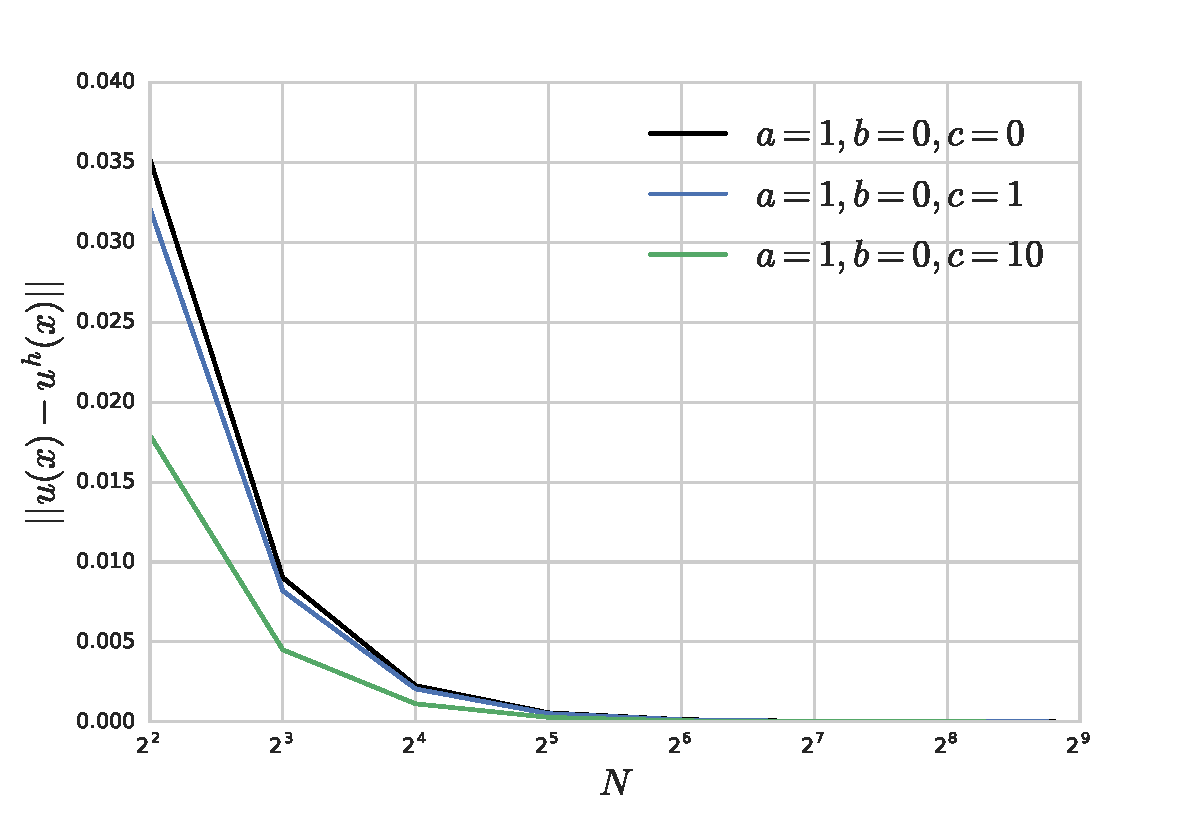
\includegraphics[width=0.75\textwidth]{img/one-d-deterministic-error.pdf}
    \caption{A plot showing the convergence of the approximations for the
             various cases}
\end{figure}

\begin{figure}
    \centering
    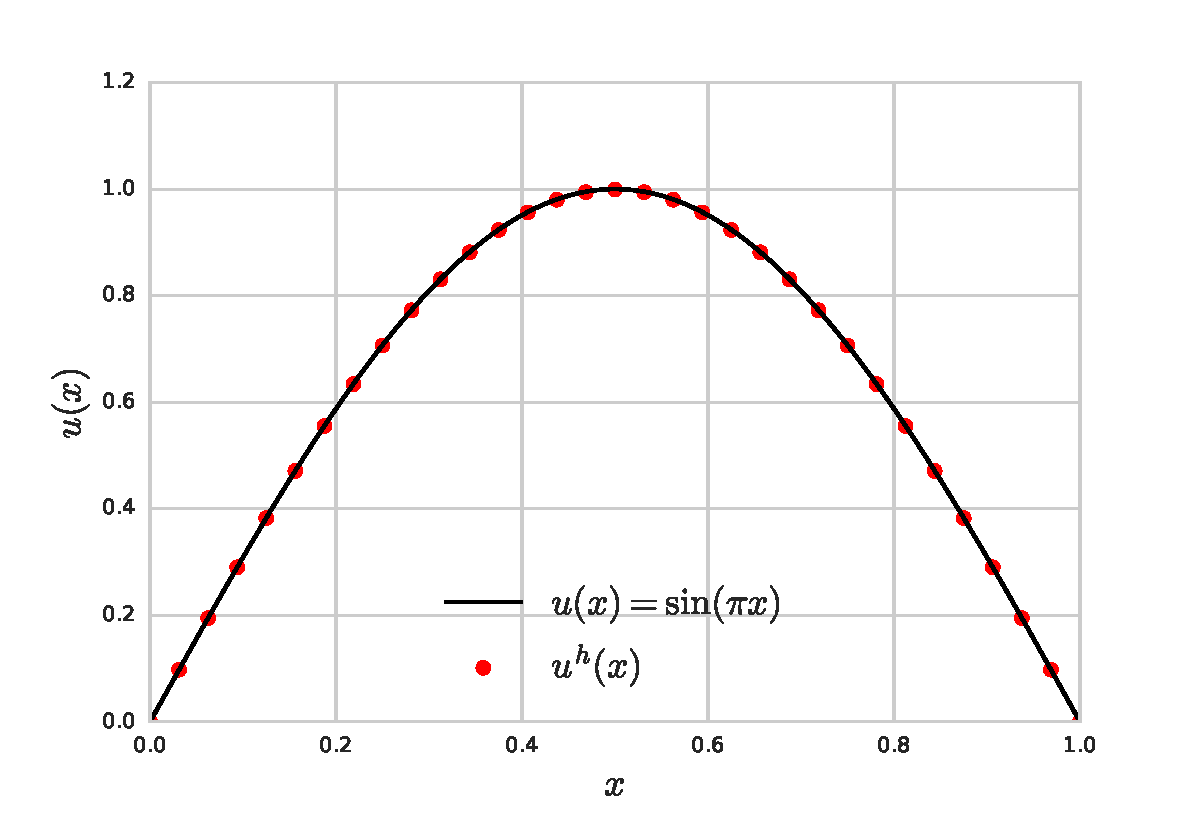
\includegraphics[width=0.75\textwidth]{img/oned-deterministic-plot.pdf}
    \caption{A plot of $u(x)$ and $u^h(x)$ in the case where $a=1, b=0, c=0$}
\end{figure}
